%%% Template originaly created by Karol Kozioł (mail@karol-koziol.net) and modified for ShareLaTeX use

\documentclass[a4paper,11pt]{article}

\usepackage[T1]{fontenc}
\usepackage[utf8]{inputenc}
\usepackage{graphicx}
\usepackage{xcolor}
\usepackage{tabularx}
\usepackage{multirow}

\usepackage{hyperref}

\renewcommand\familydefault{\sfdefault}
\usepackage{tgheros}
%\usepackage[defaultmono]{droidmono}

\usepackage{amsmath,amssymb,amsthm,textcomp}
\usepackage{enumerate}
\usepackage{multicol}
\usepackage{tikz}

\usepackage{geometry}
\geometry{left=25mm,right=25mm,%
bindingoffset=0mm, top=20mm,bottom=20mm}


\linespread{1.3}

\newcommand{\linia}{\rule{\linewidth}{0.5pt}}

% custom theorems if needed
\newtheoremstyle{mytheor}
    {1ex}{1ex}{\normalfont}{0pt}{\scshape}{.}{1ex}
    {{\thmname{#1 }}{\thmnumber{#2}}{\thmnote{ (#3)}}}

\theoremstyle{mytheor}
\newtheorem{defi}{Definition}

% my own titles
\makeatletter
\renewcommand{\maketitle}{
\begin{center}
\vspace{2ex}
{\huge \textsc{\@title}}
\vspace{1ex}
\\
\linia\\
\@author \hfill \@date
\vspace{4ex}
\end{center}
}
\makeatother
%%%

\usepackage[german]{babel}

% custom footers and headers
\usepackage{lastpage}
\usepackage{fancyhdr}
\pagestyle{fancy}
\lhead{}
\chead{}
\rhead{}
\lfoot{Tabulang Dokumentation}
\cfoot{}
\rfoot{Seite \thepage{} von \pageref{LastPage}}
\renewcommand{\headrulewidth}{0pt}
\renewcommand{\footrulewidth}{0pt}
%

% code listing settings
\usepackage{listings}
\lstset{
    language=Python,
    basicstyle=\ttfamily\small,
    aboveskip={1.0\baselineskip},
    belowskip={1.0\baselineskip},
    columns=fixed,
    extendedchars=true,
    breaklines=true,
    tabsize=4,
    prebreak=\raisebox{0ex}[0ex][0ex]{\ensuremath{\hookleftarrow}},
    frame=lines,
    showtabs=false,
    showspaces=false,
    showstringspaces=false,
    keywordstyle=\color[rgb]{0.627,0.126,0.941},
    commentstyle=\color[rgb]{0.133,0.545,0.133},
    stringstyle=\color[rgb]{01,0,0},
    numbers=left,
    numberstyle=\small,
    stepnumber=1,
    numbersep=10pt,
    captionpos=t,
    escapeinside={\%*}{*)},
    literate={ö}{{\"o}}1
           {ä}{{\"a}}1
           {ü}{{\"u}}1
}

\usepackage{tablefootnote}

%%%----------%%%----------%%%----------%%%----------%%%

\begin{document}

\title{Tabulang Docs}

\author{Wir}

\date{\today}

\maketitle

\tableofcontents
\pagebreak

\section{Parser}

Das Ziel des Parsers ist es, den Programmcode in eine Struktur zu bringen, die vom Interpreter interpretiert werden kann. Beim Lesen eines Programmcodes, wird dieser auch auf syntaktische Korrektheit überprüft. Dies geschieht mithilfe einer gegebenen Syntax in der Sprachbeschreibung.
Das Parsen wird in diesem Projekt in zwei Schritten umgesetzt. Im Unterkapitel \ref{subsection:parser} wird die Umwandlung des Programmcodes in eine Parserstruktur beschrieben. In Unterkapitel \ref{subsection:ast} wird diese dann in eine Baumstruktur gebracht, die dann an den Interpreter weiter gegeben wird. 

\subsection{Ziel}

In diesem Unterkapitel wird ein kurzer Überblick über das Ziel des Parsers gegeben. Das Schaubild \ref{fig:parseast} zeigt anhand eines kleinen Codebeispiels, wie die zwei verschiedenen Strukturen aussehen, die während des Parsens erzeugt werden. Dabei wird das Programmcodebeispiel \mbox{\textbf{x := a * (b - c) + d;}} betrachtet. Der gelbe Pfad stellt die Struktur nach dem ersten Parsen des Codes da. Dabei ist \textbf{Prg} der Wurzelknoten und \textbf{varDef} dessen einziges Statement. Im blauen Pfad mit \textbf{ProgramAST} als Wurzelknoten ist der \textbf{Abstract Syntax Tree} abgebildet. Dieser wird im weiteren Verlauf vom Interpreter verwendet.

\begin{figure}[tbh]
	%\centering
	%\hspace{-0.1\linewidth}
	%\fbox{}
	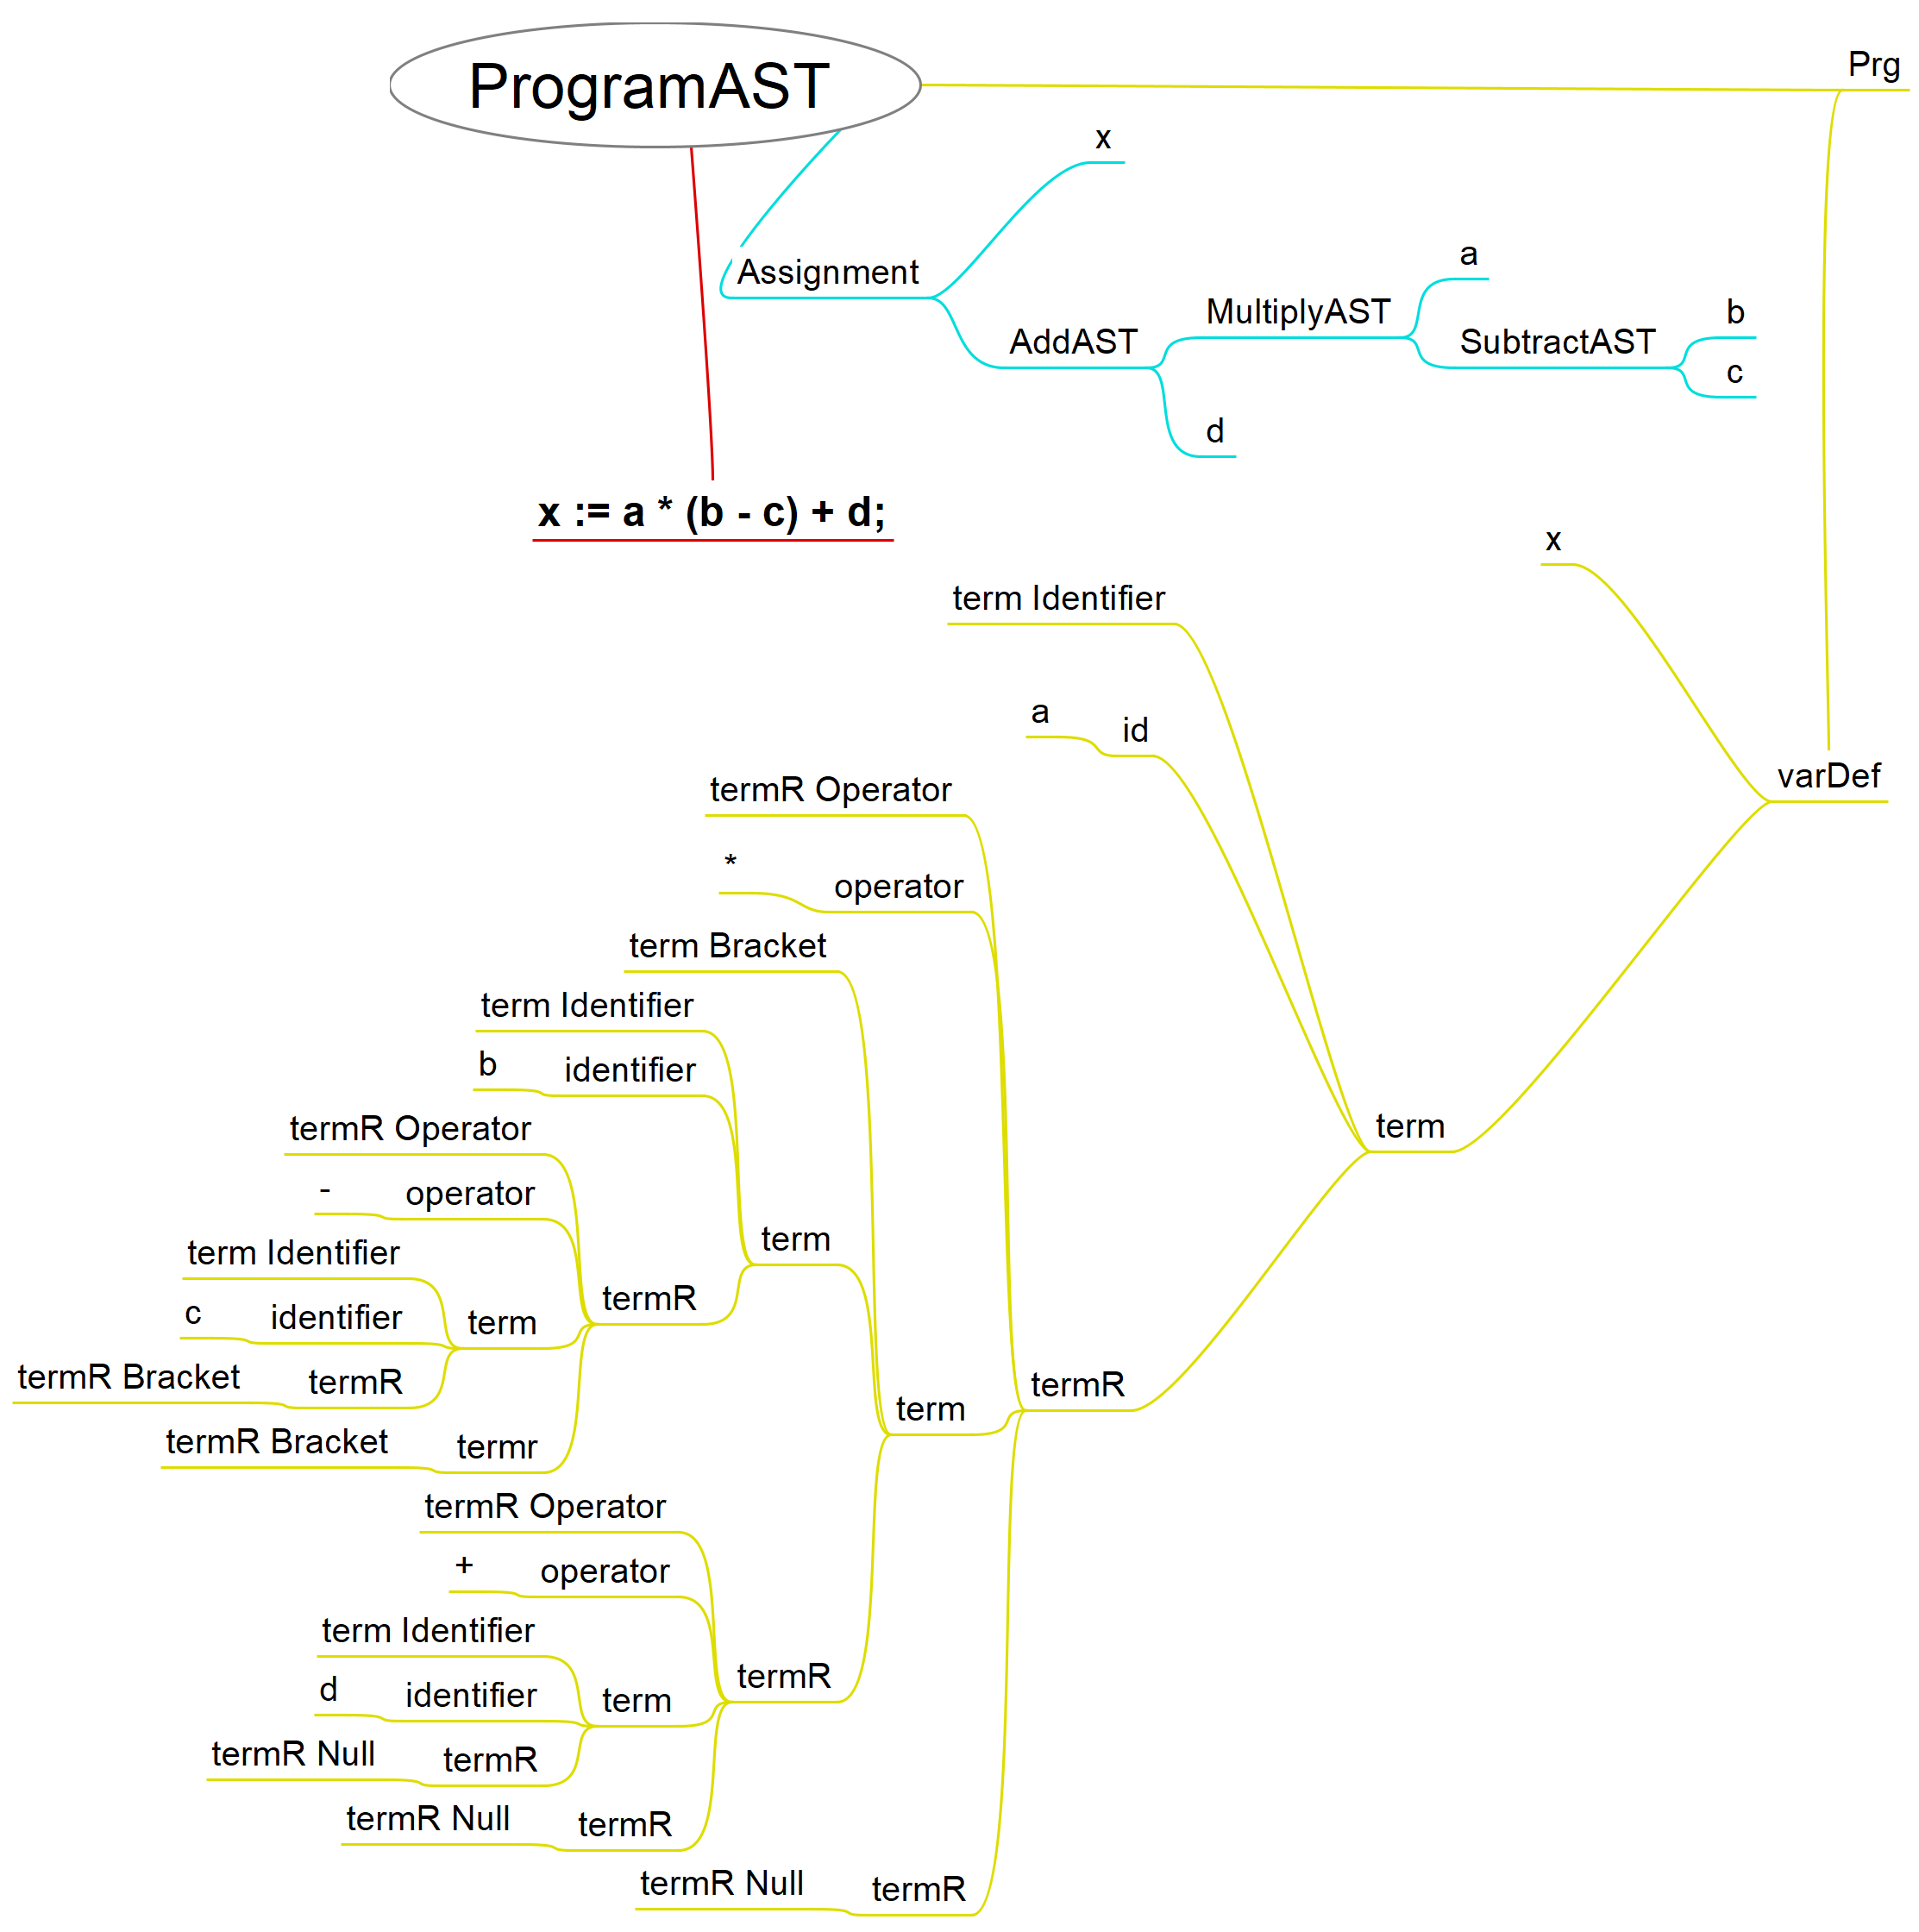
\includegraphics[width=1.0\linewidth]{images/parser-to-ast}
	\caption[Parser-Baum und AST]{Parser-Baum und AST anhand eines kleinen Beispiels}
	\label{fig:parseast}
\end{figure}

\subsection{Lexer}

Der Lexer wandelt den übergebenen Programmcode mithilfe von Regular Expressions in Tokens um. Diese enthalten jeweils den zugehörigen Text, den Typ und die Position im Text, welche später beispielsweise zum Anzeigen von Exceptions benötigt wird. 

\subsection{Parser-Baum}\label{subsection:parser}



Beim Parser-Baum handelt es sich um eine direkte Umsetzung aus der gegebenen Sprachsyntax. 
\begin{figure}[tbh]
	%\centering
	\hspace{-0.1\linewidth}
	%\fbox{}
	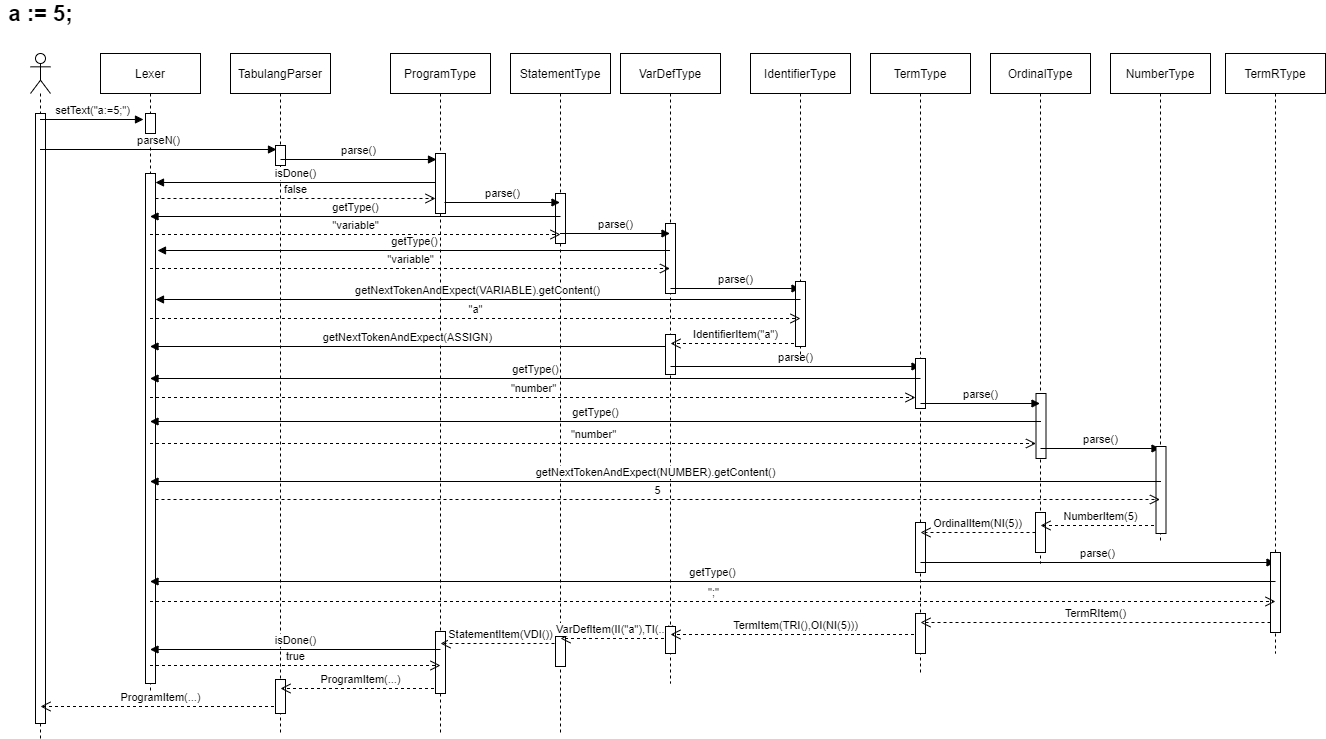
\includegraphics[width=1.2\linewidth]{images/sequenzdiagramm}
	\caption[Sequenzdiagramm Parser]{Sequenzdiagramm für die Erstellung des Parser-Baums}
	\label{fig:sequenzdiagramm}
\end{figure}


\subsection{Abstract-Syntax-Tree (AST)}\label{subsection:ast}


\pagebreak

\section{Interpreter}
\label{InterpreterIntro}
Der folgende Abschnitt beschäftigt sich mit dem Aufbau und der Funktionsweise des Interpreters. Die Aufgabe des Interpreters ist es anhand der vom \underline{Parser} erzeugten Datenstrukturen, den sogenannten Knoten (englisch: Nodes), die Semantik der Sprache korrekt zu implementieren und auszuführen. Dafür sind insbesondere zwei Klassen von Bedeutung, welche in \ref{Interpretation} und \ref{Node} vorgestellt werden.

\subsection{Die Klasse Interpretation}
\label{Interpretation}
Zuerst wird die essentielle Funktionsweise der Klasse Interpretation geklärt da diese für das Vorgehen des Interpreters wichtig ist.
Diese Klasse besitzt folgende Attribute:

\begin{lstlisting}[caption=Attribute der Klasse Interpretation, language=Java]
private Interpretation parent;
private HashMap<String, Object> environment;
private int nestingLevel;
\end{lstlisting}
Das \textbf{nestingLevel} wird hauptsächlich für die Annotatierbarkeit von Daten in einer Schleife benötigt, um das korrekte zu annotierende Datum in jeder Iteration zu bestimmen. Dies hängt eng mit dem sogenannten \textit{mapValue} zusammen, einer speziellen sprach-internen Variablen, welche für Schleifen benötigt wird. Da dies aber mehr mit der Sprache und ihren Konstrukten an sich zusammenhängt wird es hier nicht weiter konkretisiert.
\\\\
Das wohl wichtigste Attribut ist das hier genannte \textbf{environment}. Hier wird zur Laufzeit die Variablenbelegung des Programms festgehalten. Eine Zuweisung fügt dem \textbf{environment} somit entweder ein neues Schlüssel-Wert-Paar hinzu oder verändert den Wert eines bereits vorhandenen Schlüssels.

Da die Sprache Blöcke, Verschachtelungen und auch Funktionsaufrufe erlaubt, welche jeweils eine eigene Variablenbelegung besitzen können, wird eine Möglichkeit benötigt den Sichtbarkeitsbereich einer Variablen bzw. \textbf{environments}  zu beeinflussen. Dies wird durch das \textbf{parent}-Attribut realisiert. Bei jedem Aufruf eines neuen Blocks durch z. B. einer \textit{if-Anweisung}, einer \textit{for-Schleife} oder eines \textit{Funktionsaufrufs} wird eine neue Interpretation (mit leerem \textbf{environment}) erzeugt und die aktuelle Interpretation als \textbf{parent} gespeichert. Dies ermöglicht einem Block sowohl auf die Variablen der höheren Ebene(n) zuzugreifen als auch eigene lokale Variablen anzulegen welche am Ende des Blocks wieder verschwinden. 

Zudem können temporäre Interpretationen erzeugt werden, welche Zugriff auf die tatsächliche Variablenbelegung haben und dadurch bestimmte Sprachkonstrukte evaluieren können. 

Diese zwei Attribute \textbf{environment} und \textbf{parent} sind somit von zentraler Bedeutung bei der Verarbeitung und Speicherung von Variablen während der Evaluierung der vom \underline{Parser} erzeugten Datenstrukturen.
Es sollte hierbei erwähnt werden dass zu Beginn das Environment der ersten Interpretation mit den vorgefertigten Methoden aus der \underline{Standardbibliothek} befüllt wird um dem Nutzer vorab einige Funktionalitäten zur Verfügung zu stellen.


\subsection{Die Klasse Node}
\label{Node}
Bei den Datenstrukturen handelt es sich um Objekte der Klasse \textbf{Node}, genauer gesagt um die vielen Klassen welche von \textbf{Node} erben und in Baumstruktur vom \underline{Parser} bereitgestellt werden. Diese hierarchische Strukur bedeutet dass bis auf die Blätter jedes Objekt dieser Knoten weitere Knoten als Attribute hält. Jede (nicht-abstrakte) von \textbf{Node} abgeleitete Klasse implementiert folgende Methode:


\begin{lstlisting}[caption=Funktionsdeklaration der Methode \textit{evaluateNode}, language=Java]
public Object evaluateNode(Interpretation interpretation);
\end{lstlisting}
Die Funktionsweise von \textit{evaluateNode} kann grob in zwei Kategorien gliedern werden, je nachdem welche Art von Knoten sie aufruft:
\begin{itemize}
  \item Blattknoten: Gibt den Wert zurück, welcher von dem \underline{Parser} in diesem Knoten gespeichert wurde.
  \item Nicht-Blattknoten: Ruft zuerst die \textit{evaluateNode}-Methode aller der in dem Knoten gespeicherten Knoten auf und führt dann mit deren Rückgabewerten eine Operation aus.
\end{itemize}
Das Verfahren entspricht einer Art Tiefensuche beginnend mit dem Wurzelknoten bei der zuerst ein Pfad bis zu einem Blattknoten beschritten wird, welcher anschließend ein Rückgabewert an den "oberen" Knoten gibt. Hat ein Knoten alle Ergebnisse seiner Knoten erhalten wird eine Operation durchgeführt, welche von der jeweiligen Klasse abhängt. So enthält z.B. die Klasse \textbf{AddNode} zwei weitere Knoten als Attribute, dessen evaluierte Ergebnisse sie addiert.


Auf diese Weise wird Schritt für Schritt der vom Programmierer geschriebene Code ausgeführt indem der \underline{Parser} zu jedem Statement einen Syntaxbaum erzeugt welcher anschließend interpretiert wird.

\begin{figure}[H]
\centering
	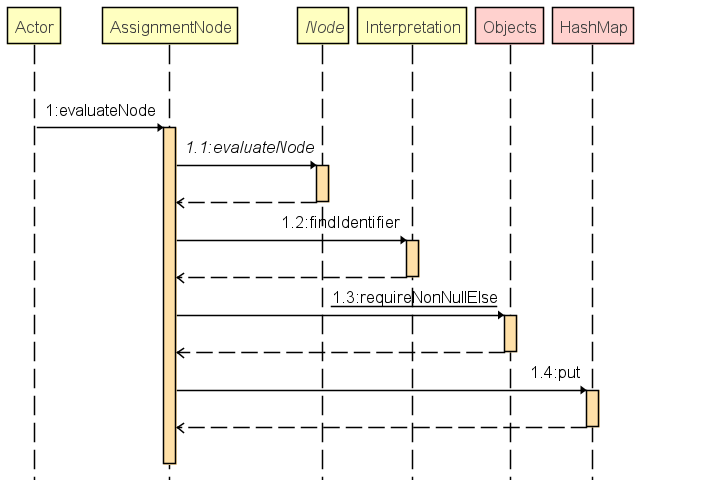
\includegraphics[width=1.1\textwidth]{images/AssignmentSequenz.png}\par\vspace{0.5cm}
	\caption{Sequenzdiagramm einer Zuweisung wie z.B. 'x := 5;'}
	\label{fig:sequence-assignment}
\end{figure}

Die oben aufgeführte Abbildung \ref{fig:sequence-assignment} zeigt den Evaluationsablauf eines Zuweisung-Statements. Ein \textbf{AssignmentNode} enthält einen weiteren Knoten, welcher zuerst evaluiert wird. Der Rückgabewert ist der zuzuweisende Wert. Als Nächstes muss geprüft werden ob der zu verwendende Identifikator bereits in einer Interpretation in Verwendung ist. Dafür wird die Methode \textit{findIdentifier} aufgerufen, welche in der aktuellen und rekursiv allen \textbf{parent} Interpretationen danach sucht. Wurde eine Interpretation gefunden, so wird der zuzuweisende Wert an die Stelle des Identifikator-Schlüssels in das \textbf{environment} geschrieben, andernfalls wird ein neues Schlüssel-Wert-Paar in das aktuelle \textbf{environment} gelegt.
\\\\
Zwischen der Klasse \textbf{Node} und den angeleiteten Klassen welche direkt vom Interpreter evaluiert werden bestehen weitere Ebenen von Knoten. Diese wurden hauptsächlich eingebaut um eine sinnvolle Gruppierung der Funktionalität zu gewährleisten und zur Reduzierung von mehrfach dupliziertem Code. So ist z.B. \textbf{BinaryArithmeticNode} eine von \textbf{ArithmeticNode} abgeleitete Klasse welche wiederum von \textbf{Node} erbt. Alle Knoten, welche für die Evaluierung von binären arithmetischen Operationen ('+', '-', '*' usw.) zuständig sind, leiten schlussendlich von dieser Klasse ab.

Durch diese Struktur kann der Interpreter in Zukunft leicht um Methoden erweitert werden, die nur von bestimmten Knoten ausgeführt werden sollen. 
Insgesamt können vom \underline{Parser} über 60 verschiedene solcher von \textbf{Node} abgeleiteten Klassen erzeugen um alle Sprachkonstrukte abzudecken und welche vom Interpreter evaluiert werden müssen. Das folgende Klassendiagramm soll zur Veranschaulichung der groben Struktur dienen. 
\begin{figure}[H]
\centering
	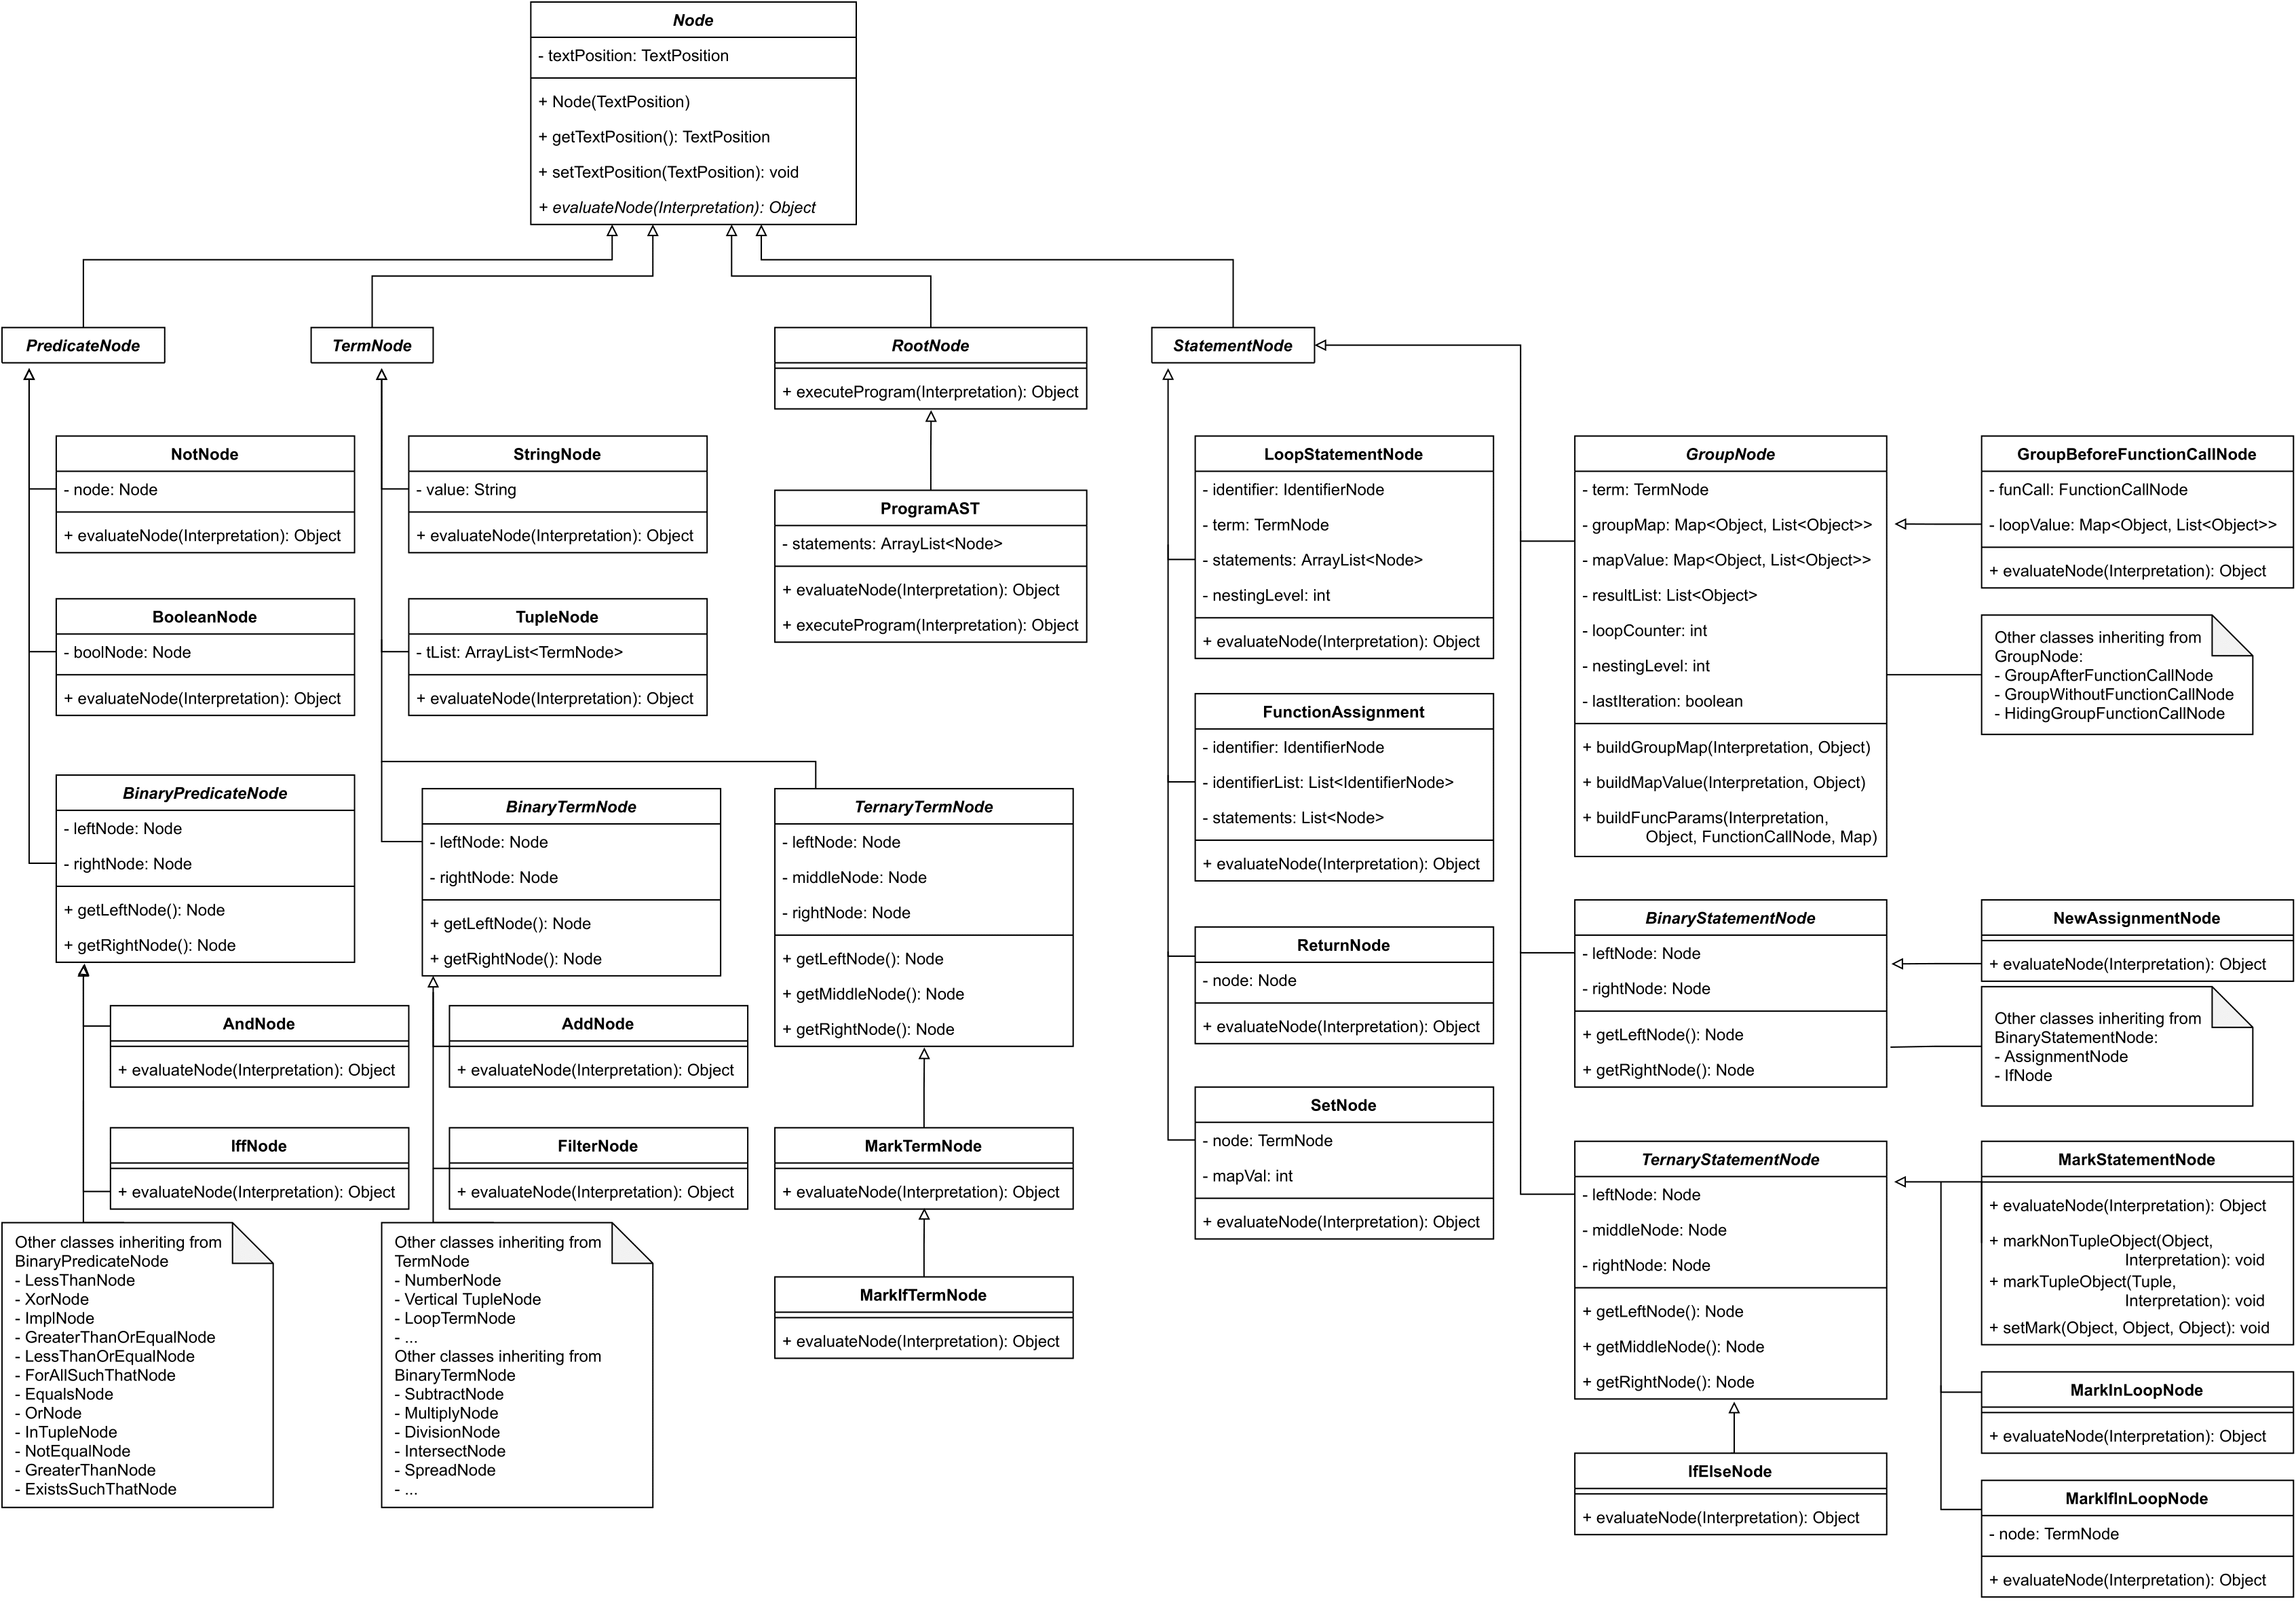
\includegraphics[width=1.1\textwidth]{images/NodeClassDiagram-1.png}\par\vspace{0.5cm}
	\caption{Klassendiagramm - Node}
\end{figure}

Es muss jedoch beachtet werden dass der \underline{Parser} nicht überprüft ob die Operanden einer Operation die korrekten \underline{Datentypen} besitzen. So kann es zur Laufzeit zu Fehlern kommen. Dies ist auch Aufgabe des Interpreters. Um dies zentral gebündelt an einer Stelle zu überprüfen enthält die Klasse \textbf{Node} zusätzlich folgende Methoden:

\begin{lstlisting}[caption=Methoden zur Typüberprüfung,label={lst:verifyMethods}, language=Java]
public Table verifyAndReturnTable(Interpretation in);
public InternalNumber verifyAndReturnNumber(Interpretation in);
public InternalBoolean verifyAndReturnBoolean(Interpretation in);
public InternalString verifyAndReturnString(Interpretation in);
public TupleOperation verifyAndReturnTupleOperation(Interpretation in);
\end{lstlisting}
Im Inneren der Funktion wird der Knoten der sie aufruft wie normal evaluiert, nur wird nach Berechnung des Ergebnisses geprüft ob dieses dem korrespondierenden \underline{Datentyp} entspricht. Wenn ja wird es zurückgegeben, wenn nicht wird eine Exception geworfen.

Jeder Knoten kann somit durch Aufruf einer dieser Methoden sicherstellen, dass die \underline{Datentypen} seiner Operanden korrekt sind. Beispiel: In einer \textbf{MultiplyNode} rufen beide Nachfolgerknoten die Methode \textit{verifyAndReturnNumber} auf um zu überprüfen dass deren Ergebnisse Zahlen sind bevor die Multiplikation ausgeführt wird. Ansonsten wird eine Fehlermeldung ausgegeben. 

Das folgende Sequenzdiagramm veranschaulicht eine korrekte Evaluierung einer \textbf{MultiplyNode}:
\begin{figure}[H]
\centering
	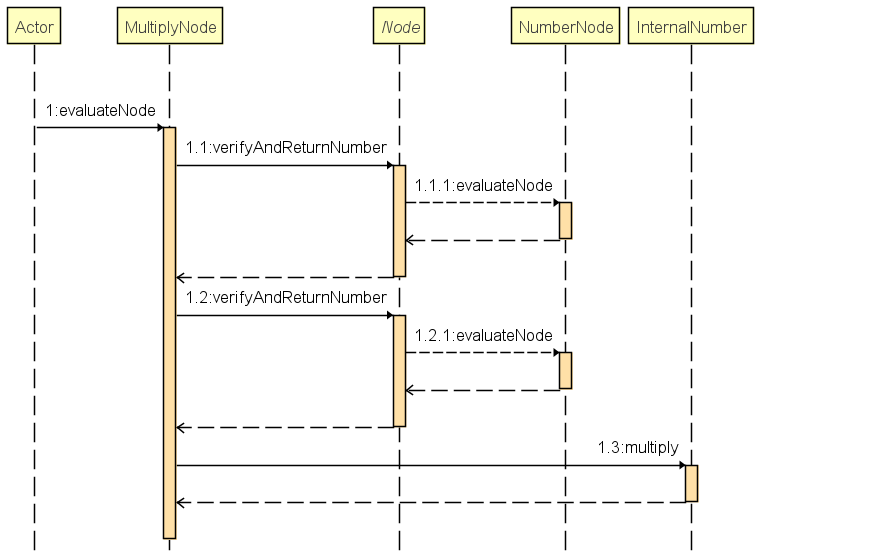
\includegraphics[width=1.1\textwidth]{images/MultiplySequenz.png}\par\vspace{0.5cm}
	\caption{Sequenzdiagramm - MultiplyNode}
\end{figure}


\subsection{Fehler während der Evaluierung}
\label{Fehlermeldungen}
Wie bereits erwähnt können zur Laufzeit des Interpreters Probleme auftreten, welche behandelt werden sollten. 
Falls während der Abarbeitung der Knoten ein Fehler auftritt, so wird eine Fehlermeldung ausgegeben. 

Um eine möglichst hilfreiche Meldung zu produzieren erhält jeder Knoten bei Erzeugung vom \underline{Parser} eine Textposition. Sollte nun bei der Ausführung der \textit{evaluateNode} eines Knotens ein Fehler auftreten, kann dem Nutzer anhand der Textposition gezeigt und markiert werden welche Zeile und Spalte des Quellcodes fehlgeschlagen ist. Des Weiteren kann jeder Knoten spezifische weitere Informationen bereitstellen weshalb eine Aktion nicht ausgeführt werden darf. Im Falle eines falschen \underline{Datentyps} werden zusätzlich die für die Operation erlaubten Operandentypen aufgelistet. Dies gilt auch für die in Listing \ref{lst:verifyMethods} aufgeführten Methoden.

\pagebreak

\pagebreak

\section{Datatypes}

Für die interne Datenhaltung und -verwaltung werden Klassen in der
Package \lstinline{datatypes} zur Verfügung gestellt. Sämtliche
interne Datentypen wie Boolean, Zahlen, Strings, Tupel, Tabellen
und Objekte erben von \lstinline{InternalObject}. So kann jede Variable, die
in Tabulang erstellt wird, annotiert und diese Annotationen durch
Aufbau einer Baumstruktur von Eltern-Objekten geerbt werden.

In diesem Kapitel wird die Umsetzung der internen Datentypen erläutert
sowie einige Fehlerbehandlungen aufgegriffen. Das Klassendiagramm in 
Abbildung \ref{fig:datatypes-uml} soll hierzu eine Übersicht über die
Zusammenhänge und die zur Verfügung gestellten Methoden geben. Zu Zwecken
der Übersicht wurden auf einige Methoden wie Getters und Setters verzichtet.

\begin{figure}[]
\centering
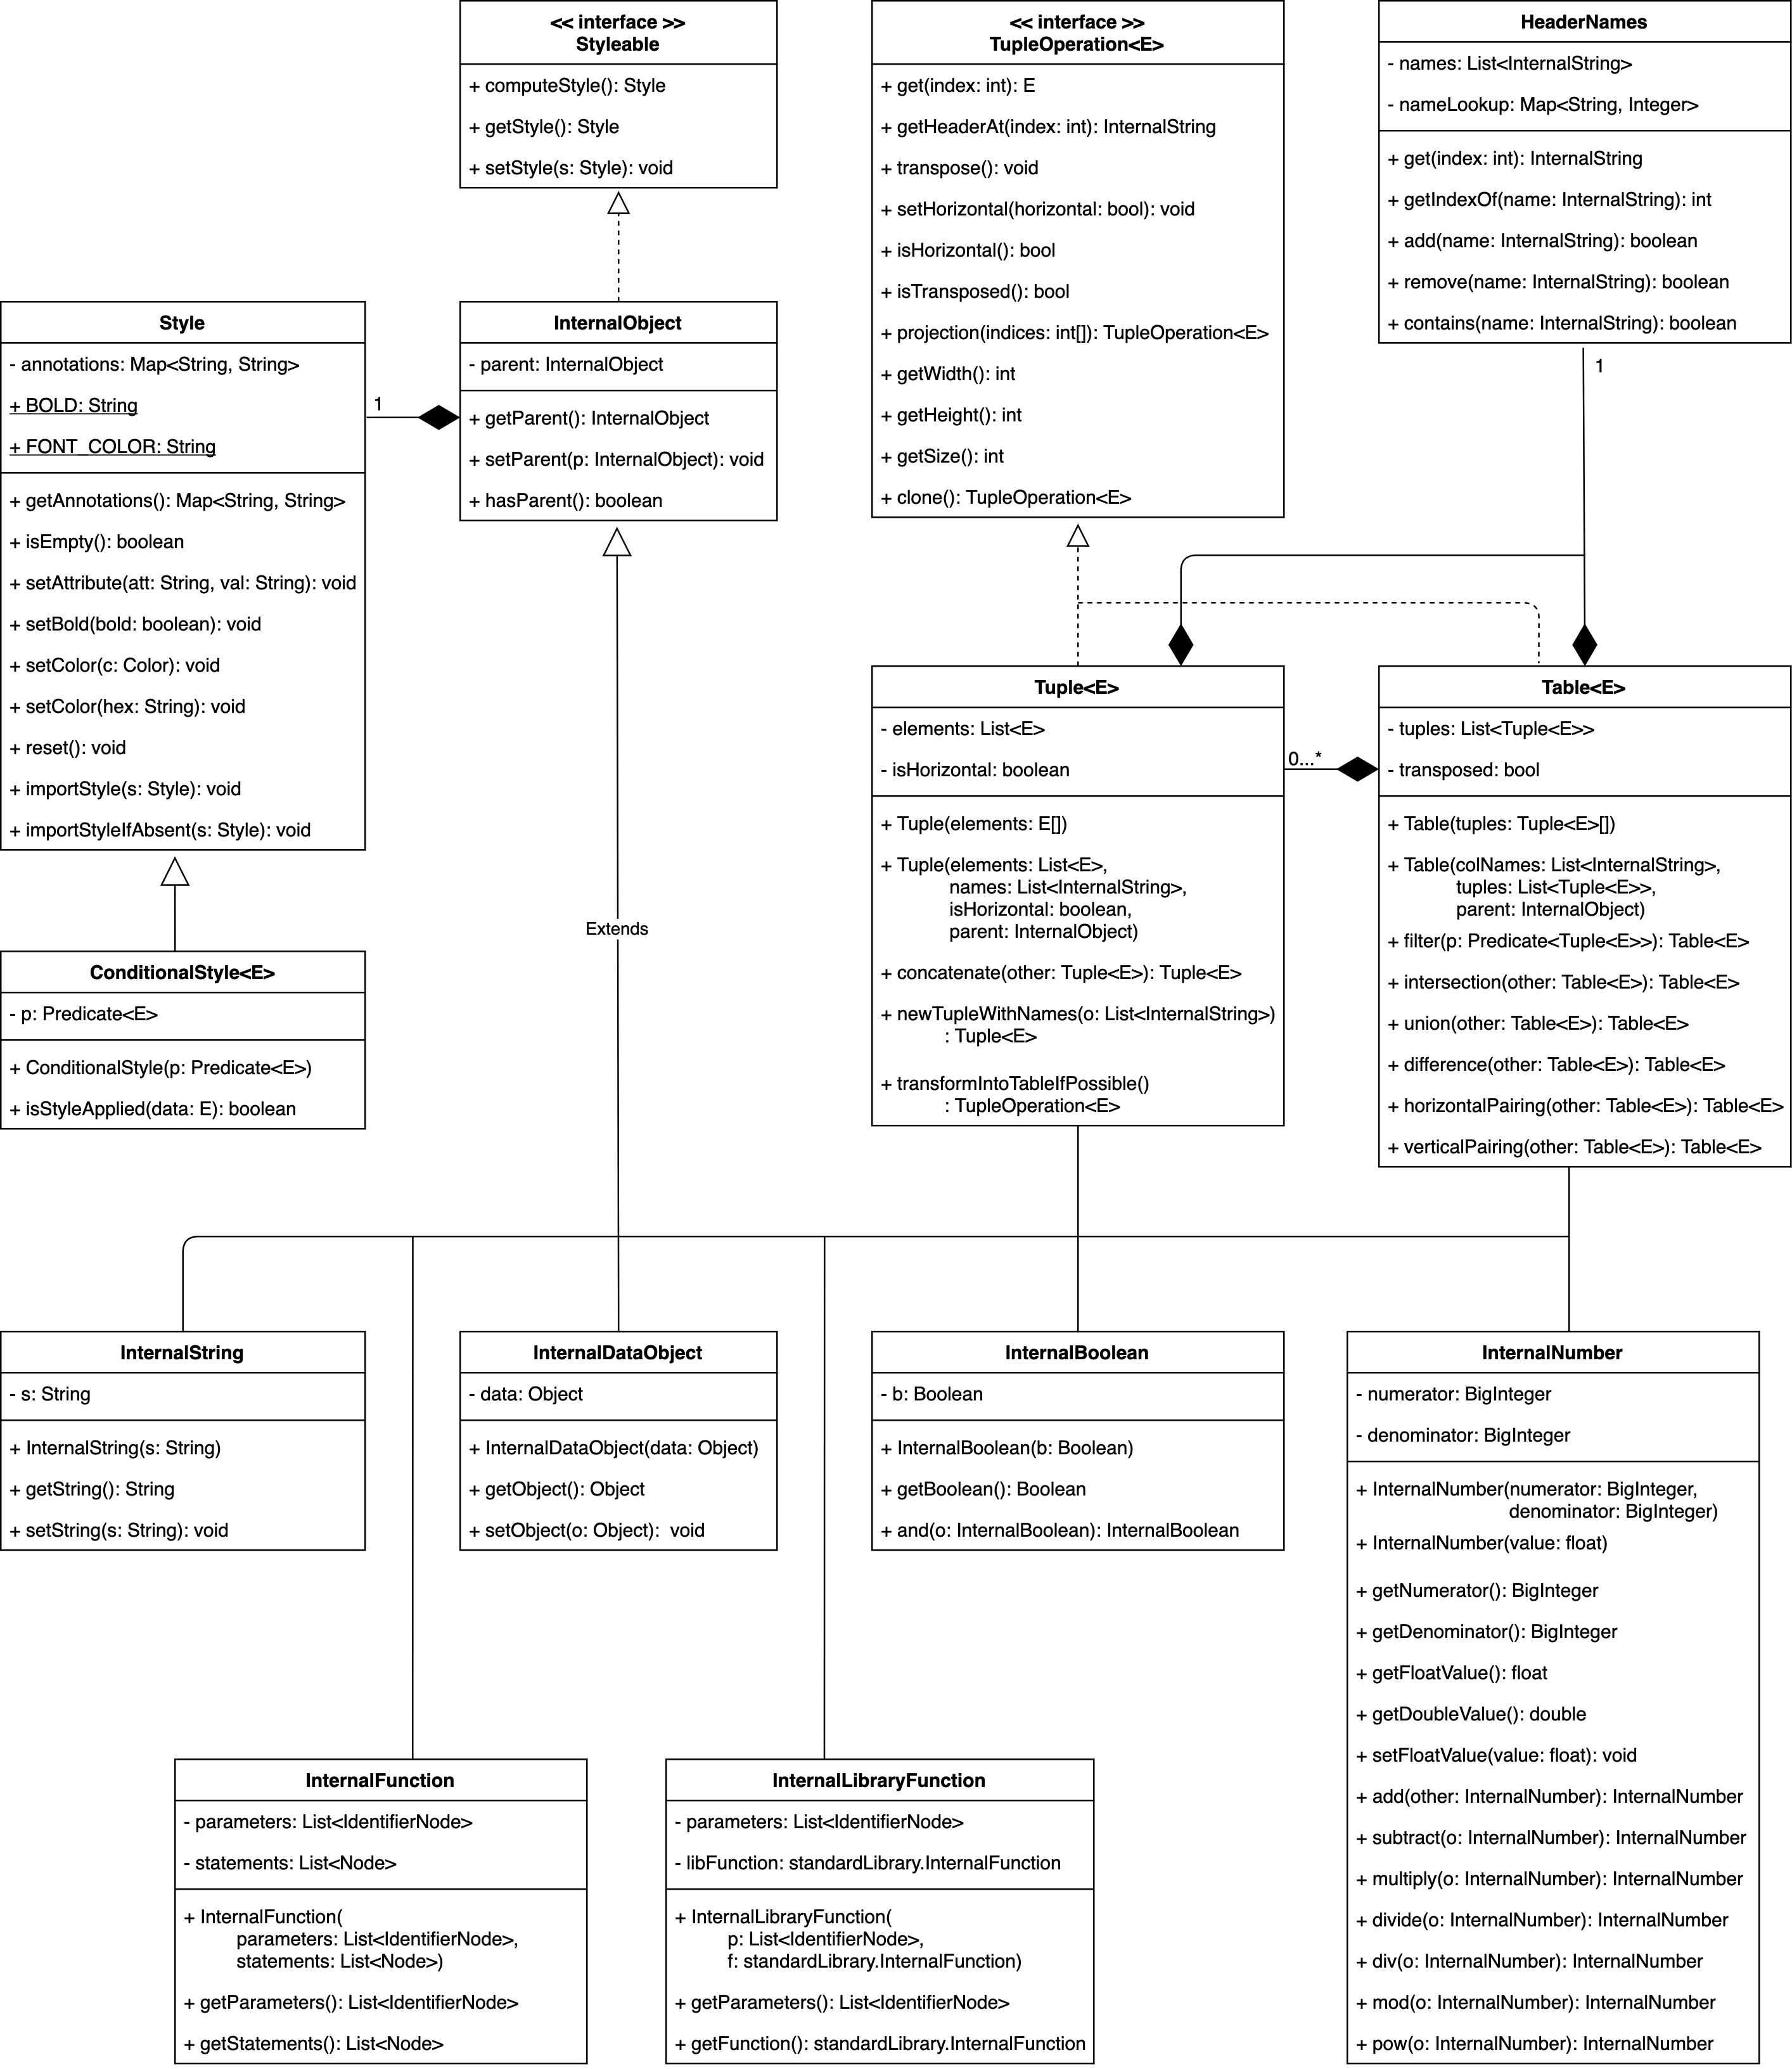
\includegraphics[width=\textwidth]{images/datatypes-uml.png}
\caption{Klassendiagramm - Datentypen}
\end{figure}\label{fig:datatypes-uml}

\subsection{Objects und Styles}

Jedes erzeugbare Objekt in Tabulang wird
in eine interne Datenhaltungsklasse gepackt,
welches die Anforderung erfüllt, alle Variable annotierbar zu machen.

Eine Annotation ist nichts anderes als ein
String-Key-Value-Paar das in einer \lstinline{map} gespeichert wird.
Mit jeder Erzeugung eines Objektes in Tabulang
wird der Variable solch eine Map angehängt, der beispielsweise
% Die zwei Leerzeichen nach dem 'bold' sind Absicht, bidde so lassen, dange
mit \lstinline{mark 'bold'  as 'true'} eine Annotation beigefügt
werden kann.

Annotationen sind vererbbar. Interne Objekte, die in Containern
enthalten sind, erben deren Annotationen, sofern bei der Vererbung keine
bereits vorhandenen Annotationen überschrieben werden.

Das Interface \lstinline{Styleable} bietet dazu lediglich die zu
implementierenden Methoden, die Klasse \lstinline{InternalObject}
die eigentliche Umsetzung. Die eigentlichen Annotationen werden in
\lstinline{Style}-Objekte gepackt.

Nachdem \lstinline{Styleable} und \lstinline{Style} recht eng miteinander
gekoppelt sind, war eine Überlegung, die Klasse \lstinline{Style}
mit den entsprechenden Methoden aus \lstinline{Styleable} abstrakt zu
machen um sich das Interface zu sparen. Es wurde sich aber aus zwei
konzeptionellen Gründen dagegen entschieden. Erstens sind Styles oder Annotationen
etwas, das Objekte \textit{besitzen} und nicht erben. Zweitens
können in Java mittels \lstinline{extends} von maximal einer Klasse geerbt
werden. Mit der Generalisierung durch einem Interface ist somit
mehr Flexibilität geboten.

\lstinline{InternalObject} bildet nun die Umsetzung der drei Methoden
\lstinline{computeStyle}, \lstinline{getStyle} und \lstinline{setStyle}.
Zusätzlich besitzt die Klasse ein \lstinline{parent} Attribut des gleichen
Typs, wodurch eine Baumstruktur von internen Objekten erzeugt werden kann.

In der Baumstruktur liegt der Hauptunterschied zwischen den Methoden \lstinline{computeStyle}
und \lstinline{getStyle}. Bei \lstinline{getStyle} wird selbsterklärend das gesetzte
\lstinline{Style}-Objekt in der Klasse zurückgegeben. In \lstinline{computeStyle}
wird ein neues \lstinline{Style}-Objekt erzeugt, dessen Annotations-Map durch das
rekursive durchhangeln durch die Elternobjekte befüllt wird. Hierbei werden nur
solche Annotationen hinzugefügt, die sich nicht bereits in der Map befinden (siehe
\lstinline{importStyleIfAbsent} in der \lstinline{Style} Klasse).\\

Die \textbf{Konstanten} in \lstinline{Style} wie zum Beispiel \lstinline{BOLD},
\lstinline{FONT_FAMILY} oder \lstinline{BACKGROUND_COLOR} werden im Wesentlichen
zum Import und Export von ods-Dateien benötigt, worauf in Kapitel \ref{subsectionLibreOffice}
eingegangen wird.

\lstinline{Style} bietet neben der Standard \lstinline{setAttribute} Methode
eine Reihe an Settern, mit der diese Konstanten gesetzt werden können. Wie sich
später aber herausstellte waren diese bis jetzt nicht sonderlich hilfreich, zumal es für
den Interpreter keine Tabulang-spezifische Konstrukte gibt, die von dem Aufruf
der Setter-Methoden profitieren könnten.

Nichtsdestotrotz wird in Listing \ref{lst:stylesetter} beispielhaft gezeigt, wie bei einem zukünftigen
Tabulang-Team diese Methoden zur Geltung kommen könnten.

\begin{lstlisting}[caption={Attribute in der Style-Klasse setzen}, label={lst:stylesetter}, language=Java]
// Diese drei Methodenaufrufe sind äquivalent
s.setStyle(Style.FONT_COLOR, "#00FF10");
s.setColor("#00FF10");
s.setColor(new Color(0, 255, 16));
\end{lstlisting}

Zu guter Letzt gab es noch die Idee, \textbf{konditionelle Styles} mittels
\lstinline{ConditionalStyle} einzuführen. Wenn in Tabulang
beispielsweise eine Variable mit \lstinline{mark 'bold'  as 'true'  if mapvalue > 0} annotiert
wird, sollte mit jedem \lstinline{computeStyle} Aufruf festgelegt werden, ob mit
dem aktuellen Wert in der Variable der Style tatsächlich gesetzt wird oder nicht.

Die genaue Umsetzung erwies sich jedoch als etwas komplizierter als erwartet. Um
eine Abfrage mittels des Predicate durchführen zu können, muss in \lstinline{computeStyle}
der aktuelle Wert bekannt sein. \lstinline{InternalObject} hat allerdings kein
Attribut, das den Wert der Variablen speichert - hierfür sind die Kindklassen vorgesehen.
Zudem ist noch nicht gewiss, wie mehrere Styles mit unterschiedlichen Konditionen innerhalb
einer Variablen gehandhabt werden sollten.

Folgende Lösungsansätze könnten in Betracht gezogen werden, die eine wesentliche Umstruktierung
der internen Datenhaltung erfordert und aus zeitlichen Gründen nicht mehr umgesetzt werden konnte.

\begin{itemize}
    \item Eine abstrakte Getter-Funktion in \lstinline{InternalObject}, die den aktuellen Wert der Variablen zurückgibt.
    \item Ein generisches Daten-Attribut in \lstinline{InternalObject}, das von den Kindklassen immer auf dem aktuellsten Stand gehalten wird.
    \item Anstelle eines Predicates werden in \lstinline{ConditionalStyle} Nodes gespeichert, die der Interpreter auswerten kann.
\end{itemize}

\subsection{Numbers}

\subsection{Tuples}

Ein Tupel ist eine geordnete Menge an Elementen, die von \lstinline{InternalObject} erben.
Tupel sind typisiert: jedem Element im Tupel wird ein String-Wert zugewiesen werden, über dem
das Element referenziert werden kann.

Die Typisierung wird über \lstinline{HeaderNames} realisiert. Das Ziel ist, den Index
eines Elements in nahezu konstanter Laufzeit zu ermitteln. Dafür spielen die zwei Attribute
\lstinline{names} (eine Liste) und \lstinline{nameLookup} (eine HashMap) in Tandem zusammen.
In \lstinline{names} wird die geordnete Menge an Strings gespeichert, in \lstinline{nameLookup}
die aktuellen Indizes der Strings.

In der Sprache kann ein Element auf zwei Arten referenziert werden, entweder über dessen typisierten Strings oder
über den Index (siehe Listing \ref{lst:tuplerefs}). Die Referenzierung wird vom Parser als \lstinline{InternalString}
übergeben. Über den Methodenaufruf \lstinline{getIndexOf(internalString)} in \lstinline{HeaderNames}
werden folgende Fälle abgearbeitet.

\begin{enumerate}
    \item Befindet sich \lstinline{internalString} in \lstinline{nameLookup}, so gebe den zugehörigen Indexwert zurück.
    \item Befindet sich \lstinline{internalString} nicht in \lstinline{nameLookup}, versuche den String in eine Zahl zu konvertieren.
    \begin{enumerate}
        \item Lässt sich \lstinline{internalString} in eine Zahl $x$ konvertieren und liegt die Zahl innerhalb des Wertebereichs $0 \leq x < \textrm{getSize()}$, gib die Zahl zurück.
        \item Sonst werfe eine \lstinline{TupleNameNotFoundException}.
    \end{enumerate}
\end{enumerate}

Namen dürfen in der Typisierung nicht doppelt erscheinen. In solchen Fällen wird eine \lstinline{DuplicateNamesException} geworfen.

Zudem sollte bei der Zuweisung einer Typisierung dieselbe Anzahl an Strings übergeben werden, die im Tupel vorhanden sind. Ansonsten
wird eine \lstinline{ArrayLengthMismatchException} geworfen.

\begin{lstlisting}[caption={Referenzierung von Tupelelementen in Tabulang}, label={lst:tuplerefs}, language=Java]
s := ['Hans', 'Peter', 67];
setHeaderNames(s, ['Vorname', 'Nachname', 'Alter']);

// beides gibt 'Peter' zurück
s.'Nachname';
s.'1';
// wirft eine TupleNameNotFoundException
s.'3';
// wirft eine DuplicateNamesException
setHeaderNames(s, ['Name', 'Name', 'Alter']);
// wirft eine ArrayLengthMismatchException
setHeaderNames(s, ['Vorname', 'Nachname', 'Alter', 'Wohnort']);
\end{lstlisting}

Ein Tupel besitzt neben den Elementen und deren Typisierung auch eine Orientierung. Diese kann auf \lstinline{horizontal} (Standard)
oder \lstinline{vertical} gesetzt werden, wie in Listing \ref{lst:tupleprint} zu sehen ist.
Die \lstinline{toString} Methode in \lstinline{Tuple} sorgt dafür, dass
je nach gegebener Ausrichtung des Tupels die Elemente gut lesbar sind.

\begin{lstlisting}[caption={Tupelausgabe mit gegebener Orientierung}, label={lst:tupleprint}, language=Java]
print(horizontal s);
// Vorname | Nachname | Alter
// Hans    | Peter    | 67
print(vertical s);
// Vorname  | Hans
// Nachname | Peter
// Alter    | 67
\end{lstlisting}

Diverse Operationen, die auf einem Tupel in der Tabulang Sprache ausgeführt werden können, sind auf die jeweiligen
Methoden in der Klasse implementiert. Der Hauptfokus lag unter Anderem darin, das Konzept einer funktionalen Programmiersprache
beizubehalten: das Tupelobjekt wird beim Aufruf einer solchen Methode nicht verändert und gibt stattdessen ein neues Objekt zurück.

In der folgenden Tabelle seien die Operationen kurz angeführt. Nachdem diese in der Sprachbeschreibung detailliert beschrieben sind, wird hier
nicht näher darauf eingegangen.

\begin{center}
    \begin{tabular}{ |l|l| } 
        \hline
        Operation & Klassenmethode \\ 
        \hline
        Änderung der Tupelorientierung & \texttt{setHorizontal(boolean horizontal)}* \\ 
        Konkatenation & \texttt{concatenate(Tuple<E> other)} \\
        Projektion & \texttt{projection(InternalString... names)} \\
        Re-Typisierung & \texttt{newTupleWithNames(List<InternalString> newNames)} \\
        \hline
    \end{tabular}
\end{center}

*Hier wird kein neues Tupelobjekt erzeugt. Stattdessen sollte \lstinline{clone()} verwendet werden und auf das geklonte Tupel die Orientierung gesetzt werden.

Exceptions, die bei diesen Operationen geworfen werden können, ähneln sich der in Listing \ref{lst:tuplerefs}. Werden
beispielsweise zwei Tupel konkateniert, die die gleiche Typisierung besitzen, wird eine \lstinline{DuplicateNamesException} geworfen.
Wird bei der Projektion ein Name nicht gefunden, wird eine \lstinline{TupleNameNotFoundException} geworfen. Bei der Re-Typisierung
könnte eine\\
\lstinline{ArrayLengthMismatchException} geworfen werden.

Letzteres bieten sowohl \lstinline{Tuple} als auch \lstinline{HeaderNames} eine Konkretisierung der Methode\\
\lstinline{iterator()}, womit
das Iterieren durch alle Elemente mittels einer for-each-Schleife möglich ist.

\subsection{Tables}

Tabellen sind im Wesentlichen Tupel, die wiederum Tupel mit jeweils gleich vielen Elementen besitzen.
Somit ähneln sich Tupel und Tabellen in ihrer Funktionsweise, weshalb die Einführung eines \lstinline{TupleOperation} Interface für sinnvoll betrachtet wurde.

Für Verwirrung könnte hier nur die Orientierung sorgen. In Tupeln spricht man davon, ob diese horizontal oder vertikal sind.
Tabellen dagegen können transponiert oder nicht transponiert sein. Wenn standardmäßig horizontale Tupel erzeugt und in eine Tabelle
gepackt werden, ist diese nicht transponiert. Wird eine Tabelle transponiert, so wird die Orientierung aller darin enthaltenen Tupel
auf vertikal gesetzt.

Nach dem selben funktionalen Schema wie bei Tupel wird mit jeder Operation auf einer Tabelle mit Ausnahme der Transponierung
ein neues Tabellenobjekt erzeugt. Auch wenn das vielleicht der sicherste Weg ist, nimmt man doch deutliche Einbußen in Leistung
und Speicherplatz hin. Für solche Zwecke wurden unter den Tests auch Benchmarks in \texttt{test/benchmarks} eingeführt, die jedoch
noch nicht sinnvoll eingesetzt werden konnten.

Im Folgenden seien die Tabellenoperationen zusammen mit ihren korrespondierenden Klassenmethoden kurz aufgeführt.
Für die detaillierte Funktionsweise wird wieder auf die Sprachbeschreibung bzw. die Dokumentation der Bibliothek gewiesen.

\begin{center}
    \begin{tabular}{ |l|l| } 
        \hline
        Operation & Klassenmethode \\ 
        \hline
        Transponierung & \texttt{transpose()}* \\ 
        Filter & \texttt{filter(Predicate<Tuple<E> > p)} \\
        Projektion & \texttt{projection(InternalString... names)} \\
        Schnitt & \texttt{intersection(Table<E> other)} \\
        Vereinigung & \texttt{union(Table<E> other)} \\
        Differenz & \texttt{difference(Table<E> other)} \\
        Horizontale Paarung & \texttt{horizontalPairing(Table<E> other)} \\
        Vertikale Paarung & \texttt{verticalPairing(Table<E> other)} \\
        \hline
    \end{tabular}
\end{center}

*Wie bei Tupel wird beim Transponieren kein neues Objekt erstellt. Stattdessen sollte man \lstinline{clone()} auf das Tabellenobjekt aufrufen und
das geklonte Objekt transponieren.

Die Filter-Methode macht sich Lambda-Funktionen aus Java 8 zunutze. So kann ein Tabellen-Objekt \lstinline{t} nach Tupeln etwa wiefolgt gefiltert werden:\\
\lstinline{t.filter(tuple -> tuple.get(new InternalString("Alter")).getFloatValue() > 18))}.

In \lstinline{intersection} wie auch in \lstinline{union} und \lstinline{difference} wird erwartet, dass beide Tabellen dieselbe Typisierung enthalten.
Ist dies nicht der Fall, wird eine \lstinline{TableHeaderMismatchException} geworfen.\\

Im Allgemeinen bietet die Sprache in Tabulang keine Möglichkeit, Tabellen zu erzeugen.
Stattdessen können Tupel von Tupel erzeugt werden, die sich weiterhin wie Tupel verhalten, bis eine Tabellenoperation darauf
ausgeführt wird. Wird etwa die Filteroperation auf ein Tupel ausgeführt, wird versucht, aus diesem Tupel eine
Tabelle zu erzeugen (siehe hierzu\\
\lstinline{transformIntoTableIfPossible} in der Klasse \lstinline{Tuple}).

Ist die Konvertierung nicht erfolgreich, bleibt das Tupel weiterhin so erhalten. In der Regel wird dann eine \lstinline{IllegalTableArgumentException} geworfen,
da eine Tabellenoperation nicht auf einem Tupel ausgeführt werden kann.

Ein volles Beispiel dazu wird in \ref{lst:tupletotable} gezeigt.

\begin{lstlisting}[caption={Tupel zu Tabellen-Konvertierung}, label={lst:tupletotable}, language=Java]
t := [['Hans','Peter'],['Amelie','Müller'],['Wilhelm','Amerson']];
setHeaderNames(t, ['p1', 'p2', 'p3']);
setHeaderNames(t.'p1', ['Vorname', 'Nachname']);
setHeaderNames(t.'p2', ['Vorname', 'Nachname']);
setHeaderNames(t.'p3', ['Vorname', 'Nachname']);

print(vertical t);
// p1 | Vorname | Nachname\\nHans    | Peter
// p2 | Vorname | Nachname\\nAmelie  | Müller
// p3 | Vorname | Nachname\\nWilhelm | Amerson

filtered := t filter stringLength(Vorname) > 5;
print(filtered);
// Vorname | Nachname
// ------------------
// Amelie  | Müller
// Wilhelm | Amerson
//
// filtered ist nun eine Tabelle
// Variable t bleibt weiterhin ein Tupel
\end{lstlisting}

\pagebreak

\section{Import Export}
\label{sectionImportExport}

Mit Hilfe dieser Implementierung ist es möglich, einen Import- bzw. Exportprozess zu starten. Diese beiden Funktionalitäten stehen für das Arbeiten mit der relationalen Datenbank \textbf{MySQL} und der Open Office Lösung \textbf{Libre Office} und dem dazugehörigen Kalkulationsprogramm \textbf{Calc} bereit. Es ist somit möglich, Daten aus einer Tabellensprache in einer MySQL-Datenbank zu archivieren und auszulesen. Außerdem können Daten aus einer *.ods-Datei, die das Dateiformat von Libre Office Calc darstellt, ausgelesen werden. Ferner kann aus der Tabellensprache eine *.ods-Datei generiert werden. In den nächsten zwei Unterkapiteln \ref{subsectionMySql} und \ref{subsectionLibreOffice} werden die einzelnen Kernfunktionalitäten näher erläutert.

\subsection{MySQL}
\label{subsectionMySql}

\subsubsection{Models}
\label{subsubsectionMySqlModels}
\textbf{MSqlConnectionParameters}

\begin{lstlisting}[label={labelMySqlConnectionParameters},caption=Parameter für eine MySQL-Datenbankverbindung, language=Java]
private String _ip;
private int _port;
private String _dbName;
private String _username;
private String _password;
\end{lstlisting}

\textbf{MSqlTableContent}

\begin{lstlisting}[label={labelMySqlConnectionParameters},caption=Repräsentation einer MySQL-Tabelle als Java-Objekt, language=Java]
private String _dbName;
private ArrayList<String> _headlines;
private ArrayList<ArrayList<String>> _content;
\end{lstlisting}

\subsubsection{Öffentliche Funktionen}
\label{subsubsectionMySqlPublicFunctions}

\subsubsection{Private Funktionen}
\label{subsubsectionMySqlPrivateFunctions}

\subsection{Libre Office}
\label{subsectionLibreOffice}

\subsubsection{Models}
\label{subsubsectionLibreOfficeModels}

\textbf{MCell}

\begin{lstlisting}[label={labelMySqlConnectionParameters},caption=Repräsentation einer Zelle einer Libre Office Calc Datei, language=Java]
private HashMap<String,String> Attributes;
private Object _value;
\end{lstlisting}

\textbf{MColumn}

\begin{lstlisting}[label={labelMySqlConnectionParameters},caption=Repräsentation einer Spalte einer Libre Office Calc Datei, language=Java]
private HashMap<String,String> Attributes;
\end{lstlisting}

\textbf{MRow}

\begin{lstlisting}[label={labelMySqlConnectionParameters},caption=Repräsentation einer Zeile einer Libre Office Calc Datei, language=Java]
private HashMap<String,String> Attributes;
private ArrayList<Cell> _cells;
\end{lstlisting}

\textbf{MSpreadsheet}

\begin{lstlisting}[label={labelMySqlConnectionParameters},caption=Repräsentation einer kompletten Libre Office Calc Datei, language=Java]
private ArrayList<HashMap<String, String>> _fontStyles;
private HashMap<String, HashMap<String, String>> _tableStyles;
private HashMap<String, HashMap<String, String>> _rowStyles;
private HashMap<String, HashMap<String, String>> _columnStyles;
private HashMap<String, HashMap<String, String>> _cellStyles;
private ArrayList<TableWrapper> _tables;
\end{lstlisting}

\textbf{MStyle}

\begin{lstlisting}[label={labelMySqlConnectionParameters},caption=Repräsentation eines Styles einer Libre Office Calc Datei, language=Java]
private OdfStyleProperty property;
private String value;
\end{lstlisting}

\textbf{MTableWrapper}

\begin{lstlisting}[label={labelMySqlConnectionParameters},caption=Repräsentation einer Tabelle einer Libre Office Calc Datei inkl. aller Zeilen und Spalten, language=Java]
private HashMap<String,String> _attributes;
private ArrayList<Column> _columns;
private ArrayList<Row> _rows;
\end{lstlisting}

\subsubsection{Öffentliche Funktionen}
\label{subsubsectionLibreOfficePublicFunctions}

\subsubsection{Private Funktionen}
\label{subsubsectionLibreOfficePrivateFunctions}
\pagebreak

\section{Extras}

\subsection{Standardbibliothek}\label{sectionStandardBibliothek}

Mithilfe interner Funktionen soll die Klippe zwischen Sprache und Systemoperationen überbrückt werden.
In der Package \texttt{standardLibrary} werden diese internen Funktionen in Java umgesetzt.

Dabei implementiert jede interne Standardbibliotheksfunktion die Methode \\
\texttt{compute(Object... objects)} aus dem Interface \texttt{InternalFunction}.
Die jeweilige Implementierung wird zusammen mit den geforderten Parametern und einem Funktionsnamen vor dem Start des Interpreters in dessen Environment gepackt.
Wird aus Tabulang die entsprechende interne Funktion wie zum Beispiel \texttt{print(123)} aufgerufen, wird im Interpreter die korrekte Anzahl der Parameter überprüft und mit dem Aufruf der \texttt{compute} Methode die entsprechende interne Funktion ausgeführt.

In Abbildung \ref{fig:standardlib-uml} wird zusätzlich gezeigt, wie die statischen Methoden in \texttt{StandardLibrary} durch alle verfügbaren Funktionsklassen geht, ein Objekt davon erstellt und dieses dem Interpreter hinzufügt.

\begin{figure}[h]
\centering
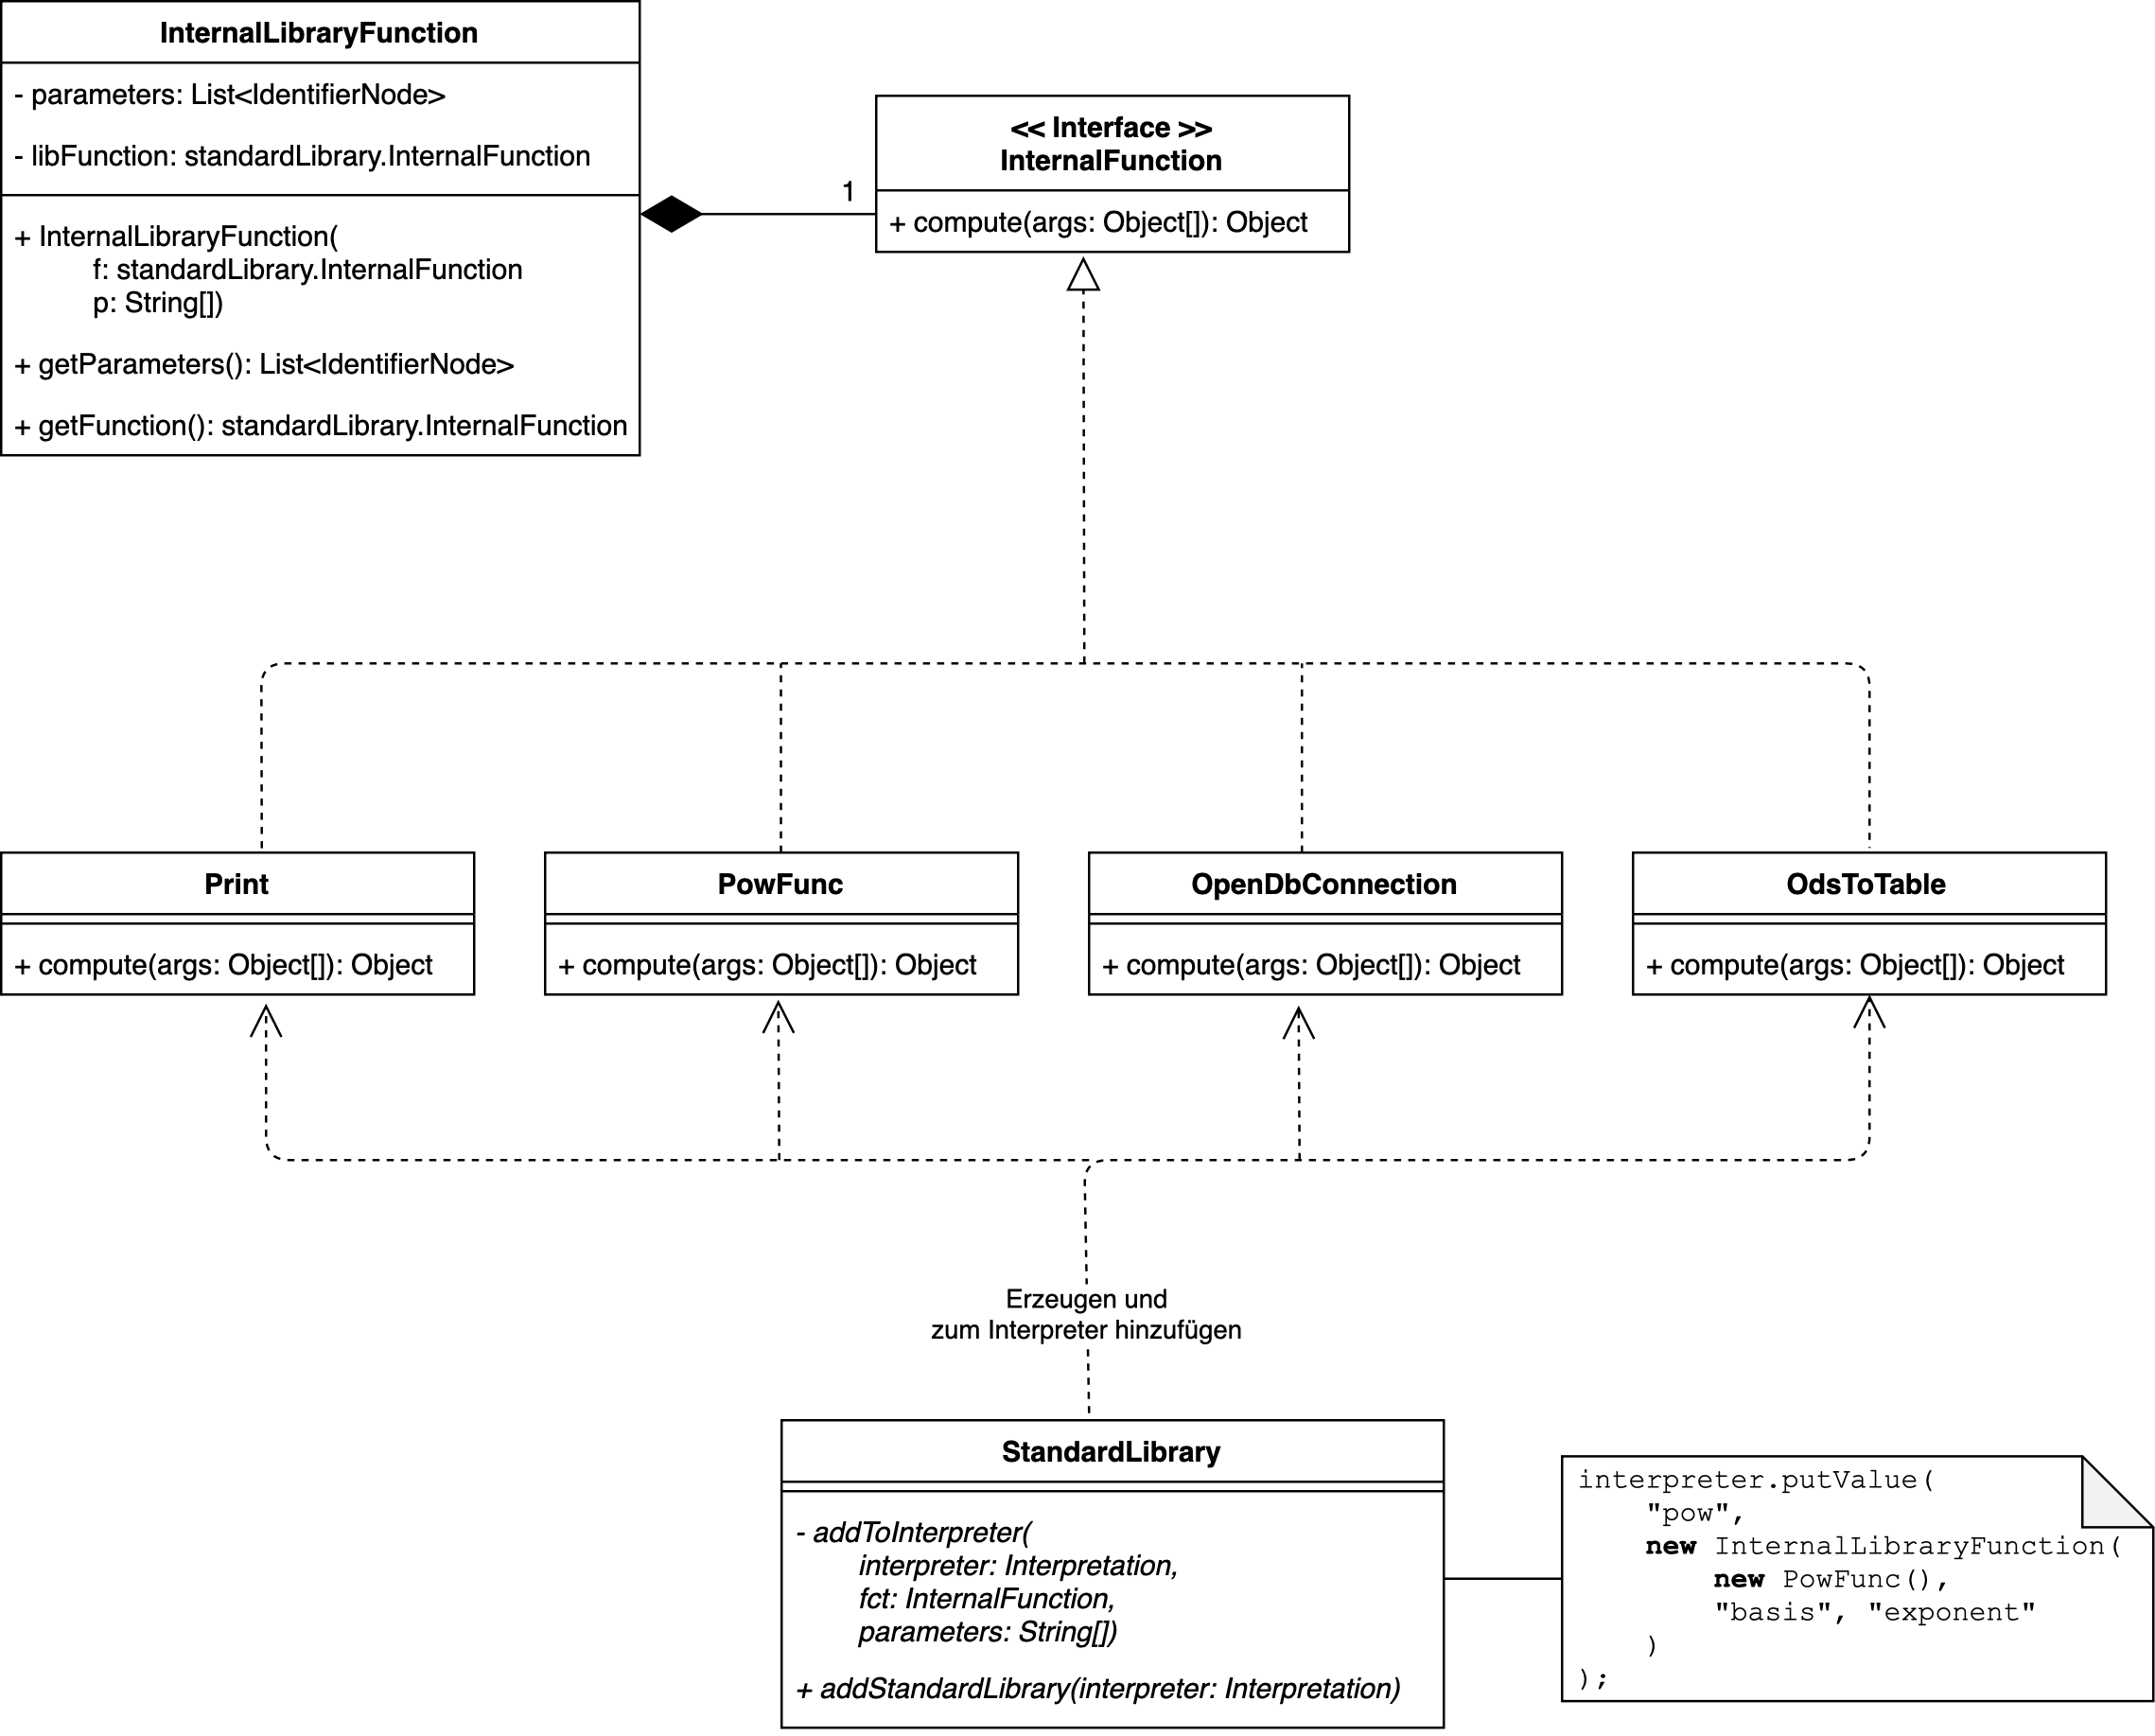
\includegraphics[width=.8\textwidth]{images/standardlib-uml.png}
\caption{Klassendiagramm - Standardbibliothek}
\end{figure}\label{fig:standardlib-uml}

\subsection{VS Code Extension}

Als Proof-of-Concept wurde eine Visual Studio Code Extension erstellt, die die Schlüsselwörter aus Tabulang farblich hervorhebt.
Die dafür benötigten Dateien befinden sich im Ordner \texttt{vscode extension}.

Um von der Extension Gebrauch machen zu können, wird auf die Datei\\
\texttt{vsc-extension-quickstart.md} verwiesen.
Weiterführend kann an der Extension mithilfe der offiziellen Dokumentation von VS Code weitergearbeitet werden: https://code.visualstudio.com/api/language-extensions/overview

\end{document}
